\let\negmedspace\undefined
\let\negthickspace\undefined
\documentclass[journal]{IEEEtran}
\usepackage[a5paper, margin=10mm, onecolumn]{geometry}
%\usepackage{lmodern} % Ensure lmodern is loaded for pdflatex
\usepackage{tfrupee} % Include tfrupee package

\setlength{\headheight}{1cm} % Set the height of the header box
\setlength{\headsep}{0mm}     % Set the distance between the header box and the top of the text

\usepackage{gvv-book}
\usepackage{gvv}
\usepackage{cite}
\usepackage{amsmath,amssymb,amsfonts,amsthm}
\usepackage{algorithmic}
\usepackage{graphicx}
\usepackage{textcomp}
\usepackage{xcolor}
\usepackage{txfonts}
\usepackage{listings}
\usepackage{enumitem}
\usepackage{mathtools}
\usepackage{gensymb}
\usepackage{comment}
\usepackage[breaklinks=true]{hyperref}
\usepackage{tkz-euclide} 
\usepackage{listings}
% \usepackage{gvv}                               

\def\inputGnumericTable{}                      
\usepackage[latin1]{inputenc}                    
\usepackage{color}                              
\usepackage{array}                             
\usepackage{longtable}                          
\usepackage{calc}                               
\usepackage{multirow}                           
\usepackage{hhline}                            
\usepackage{ifthen}                          
\usepackage{lscape}
\begin{document}

\bibliographystyle{IEEEtran}
\vspace{3cm}

\title{2.6.35}
\author{AI25BTECH11024 - Pratyush Panda
}
\maketitle
% \newpage
% \bigskip
{\let\newpage\relax\maketitle}

\renewcommand{\thefigure}{\theenumi}
\renewcommand{\thetable}{\theenumi}
\setlength{\intextsep}{10pt} % Space between text and floats


\numberwithin{equation}{enumi}
\numberwithin{figure}{enumi}
\renewcommand{\thetable}{\theenumi}

\textbf{Question: } \\
The value of $\hat{\Vec{i}}.\brak{\hat{\Vec{j}} \times \hat{\Vec{k}}} + \hat{\Vec{j}}.\brak{\hat{\Vec{i}} \times \hat{\Vec{k}}} + \hat{\Vec{k}}.\brak{\hat{\Vec{i}} \times \hat{\Vec{j}}}$ is \underline{\hspace{2cm}}
\vspace{0.5cm}

\textbf{Solution: } \\
Given:
\begin{align}
\Vec{\hat{i}}=\Vec{e_1}=\myvec{1 \\ 0 \\ 0}, \, \Vec{\hat{j}}=\Vec{e_2}=\myvec{0 \\ 1 \\ 0}, \, \Vec{\hat{k}}=\Vec{e_3}=\myvec{0 \\ 0 \\ 1}
\end{align}

Each term of the expression in the question can be found using the scalar triple product determinant.\\
The first term can be written as:
\begin{align}
\brak{\hat{\Vec{i}}.\brak{\hat{\Vec{j}} \times \hat{\Vec{k}}}} = 
\myvec{e_1 && e_2 && e_3} =
\myvec{1 && 0 && 0 \\
       0 && 1 && 0 \\
       0 && 0 && 1}
\end{align}
Determinant of this matrix is 1. Thus, the value of first term is 1.

The second term can be written as:
\begin{align}
\brak{\hat{\Vec{j}}.\brak{\hat{\Vec{i}} \times \hat{\Vec{k}}}} = 
\myvec{e_2 && e_3 && e_1} =
\myvec{0 && 0 && 1 \\
       1 && 0 && 0 \\
       0 && 1 && 0}
\end{align}
Determinant of this matrix is -1. Thus, the value of first term is -1.

The third term can be written as:
\begin{align}
\brak{\hat{\Vec{k}}.\brak{\hat{\Vec{i}} \times \hat{\Vec{j}}}} = 
\myvec{e_3 && e_1 && e_2} =
\myvec{0 && 1 && 0 \\
       0 && 0 && 1 \\
       1 && 0 && 0}
\end{align}
Determinant of this matrix is 1. Thus, the value of first term is 1.

So, the sum of all the terms is;
\begin{align}
\hat{\Vec{i}}.\brak{\hat{\Vec{j}} \times \hat{\Vec{k}}} + \hat{\Vec{j}}.\brak{\hat{\Vec{i}} \times \hat{\Vec{k}}} + \hat{\Vec{k}}.\brak{\hat{\Vec{i}} \times \hat{\Vec{j}}} = 1 + (-1) + 1
\end{align}
\begin{align}
or, \, \hat{\Vec{i}}.\brak{\hat{\Vec{j}} \times \hat{\Vec{k}}} + \hat{\Vec{j}}.\brak{\hat{\Vec{i}} \times \hat{\Vec{k}}} + \hat{\Vec{k}}.\brak{\hat{\Vec{i}} \times \hat{\Vec{j}}} = 1
\end{align}

\begin{figure}[H]
\centering
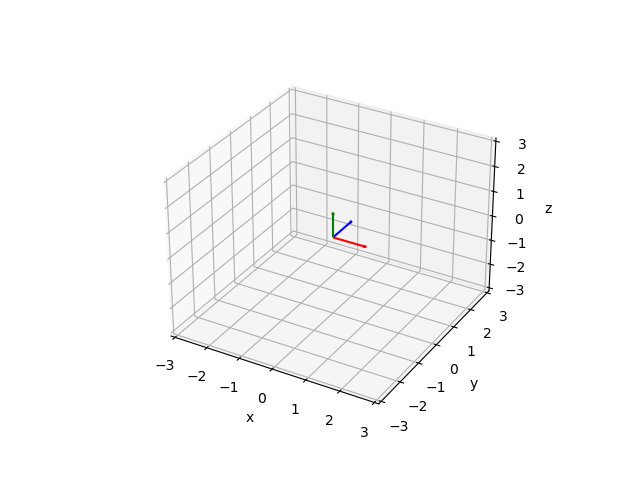
\includegraphics[width=0.6\columnwidth]{figs/img.png}
\caption*{}
\end{figure}

\end{document}
